\chapter{Compensators}
Compensators modify the loop transfer function $L(s)$ of a feedback system to stabilize the system or improve its performance.
Compensators add one or more poles and/or zeros to $L(s)$ to change the feedback system's steady-state error, noise rejection, crossover frequency $\omega_{c}$, phase margin $\phi_{M}$, gain margin, etc.
There are three types of compensators: lag, lead, and lead-lag compensators.

Lag compensators have a low frequency pole and a higher frequency zero so they have a transfer function of the form \[G_{c}(s) = K\frac{\tau_{1}s+1}{\tau_{2}s+1}, \tau_{1} < \tau_{2}\]
Lag compensators are typically used either to decrease $|L(s)|$ at high frequencies while maintaining a high $|L(s)|$ at low frequencies, or to increase $|L(s)|$ at low frequencies without also increasing $|L(s)|$ at high frequencies.
The latter is more common, and decreases the system's steady state error and improves its disturbance rejection but maintains $\omega_{c}$, $\phi_{M}$, and (high frequency) noise rejection. \autocite[269]{analog-design-feedback-lundberg}

Lead compensators have a low frequency zero and high frequency pole so a lead compensator's transfer function is of the form \[G_{c}(s) = K\frac{\alpha \tau_{1}s+1}{\tau_{2}s+1}, \tau_{1} > \tau_{2}\]
The phase increases (i.e. moves away from $-\pi$) between the zero and pole's frequency, so $\phi_{M}$ can be increased if the zero and pole are placed such that $\omega_{c}$ is greater than the zero's frequency but less than the pole's frequency.
The maximum increase in phase between the compensator's zero and pole is given by $\phi = \arcsin \frac{\alpha - 1}{\alpha + 1}$.
A typical value of $\alpha = 10$ yields $\phi = 55\,^{\circ}$.
$\alpha$ should not be too high, however, because the higher the value of $\alpha$ the greater the increase in high frequency gain (which reduces high frequency noise rejection).
The easiest way to design a lead compensator is to place the zero at $\omega_{c}$ -- if $\alpha$ is high enough (i.e. the pole is at a high enough frequency) the phase margin $\phi_{M}$ can be increased by approximately $45\,^{\circ}$ and $\omega_{c}$ is not changed significantly.
To maximize the increase in $\phi_{M}$, however, the zero and pole should be placed such that their geometric mean is equal to $\omega_{c}$. \autocite[277-278]{analog-design-feedback-lundberg}

The benefits of both a lead and lag compensator can be acheived with a lead-lag compensator, which can be as simple as cascading a lag compensator and lead compensator.
The lag compensator can improve the low frequency characteristics of the plant while the lead compensator improves the plant's transfer function near $\omega_{c}$.

\section{Passive lag compensator}
\begin{center}
	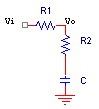
\includegraphics{schematics/passivelag.PNG}
\end{center}
This lag compensator is constructed out of passive components. It cannot achieve a gain greater than 1 (i.e. $K > 1$), of course, but in cases where such a gain is not necessary this compensator can reduce the feedback system's power consumption versus an active lag compensator. It is easy to see how this is a lag compensator: at low frequencies the capacitor is an open circuit so the impedance to ground is much higher than $R_{1}$ and $\frac{v_{o}}{v_{i}}(s) = 1$, and at high frequencies the capacitor is a short so $R_{1}$ and $R_{2}$ form a simple voltage divider which gives $\frac{v_{o}}{v_{i}}(s) = \frac{R_{2}}{R_{1}+R_{2}}$. To be more precise, this is a voltage divider consisting of impedances $R_{1}$ and $R_{2}+\frac{1}{sC}$. The transfer function \autocite[270]{analog-design-feedback-lundberg} is therefore

\textcolor{red}{
\begin{equation}
\frac{\vout}{\vin}(s) = \frac{R_2+\frac{1}{sC}}{R_1 + R_2 + \frac{1}{sC}} = \frac{sR_2 C + 1}{1+s(R_1 + R_2)C}
\label{eq:passivelagcompensator}
\end{equation}
}

An alternative passive lag compensator places the capacitor in parallel with $R_2$ rather than in series with it:
\begin{figure}[h]
	\centering
		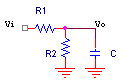
\includegraphics{schematics/passivelag2.PNG}
	\caption{Alternative passive lag compensator}
	\label{fig:passivelag2}
\end{figure}

This too is a voltage divider, but this time the impedances are $R_1$ and $R_2 \parallel C$.
The transfer function is $\frac{\vout}{\vin}(s) = \frac{R_2 \parallel C}{R_1 + R_2 \parallel C} = \frac{R_2}{R_1 + R_2 +sR_1 R_2 C}$, which is best expressed as

\textcolor{red}{
\begin{equation}
\frac{\vout}{\vin}(s) = \frac{R_2}{R_1 + R_2}\frac{1}{1+s(R_1 \parallel R_2)C}
\end{equation}
}

to make the DC gain and the location of the pole obvious.

\section{Passive lead compensator}
\begin{center}
	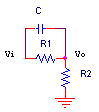
\includegraphics{schematics/passivelead.PNG}
\end{center}
This lead compensator is very similar to the above passive lag compensator. In this case, at low frequencies the capacitor is an open circuit so $R_{1}$ and $R_{2}$ simply form a voltage divider to give $\frac{v_{o}}{v_{i}}(s) = \frac{R_{2}}{R_{1}+R_{2}}$, and at high frequencies the capacitor shorts $R_{1}$ so that $\frac{v_{o}}{v_{i}}(s) = 1$. The full analysis isn't much more difficult: this is an voltage divider consisting of impedances $R_{1}||\frac{1}{sC} = \frac{R_{1}}{1+sR_{1}C}$ and $R_{2}$. The transfer function is thus

\textcolor{red}{
\begin{equation}
\frac{v_{o}}{v_{i}}(s) = \frac{R_{2}}{\frac{R_{1}}{sR_{1}C+1} + R_{2}} = \frac{R_{2}(sR_{1}C + 1)}{(R_{1} + R_{2})(s\frac{R_{1}R_{2}}{R_{1}+R_{2}}C + 1)}
\label{eq:passivelead}
\end{equation}
}

The latter expression puts the transfer function in the $K\frac{\alpha \tau_1 s+1}{\tau_2 s+1}$ form to make the gain and time constants clear. \autocite[278]{analog-design-feedback-lundberg}

\section{Passive lead-lag compensator}
\begin{center}
	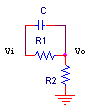
\includegraphics{schematics/passiveleadlag.PNG}
\end{center}
This lead-lag compensator provides the benefits of both a lead compensator and a lag compensator and does it entirely with passive components. Its transfer function is fairly easy to derive since this circuit is a voltage divider using the impedances $R_1 \parallel \frac{1}{sC}$ and $R_2$.
Since

\begin{equation}
R_1 \parallel C = \frac{R_1}{1+sR_1 C}
\end{equation}
we have
\begin{equation}
\frac{\vout}{\vin}(s) = \frac{R_2}{R_2 + \frac{R_1}{1+sR_1 C}} = \frac{R_2(1+sR_1 C)}{R_1 + R_2 + sR_1 R_2 C}
\end{equation}

By factoring out $R_1 + R_2$ we get

\textcolor{red}{
\begin{equation}
\frac{\vout}{\vin}(s) = \frac{R_2}{R_1 + R_2}\frac{1+sR_1 C}{1+s(R_1 \parallel R_2)C}
\label{eq:passiveleadlag}
\end{equation}
}

The location of the zero is determined first by choosing appropriate values of $R_1$ and $C$, and $R_2$ determines the location of the pole.

\section{Active lag compensator}
\begin{center}
	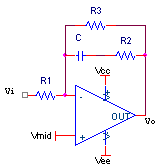
\includegraphics{schematics/activelag.PNG}
\end{center}
This is a basic lag compensator constructed with an operational amplifier so that a choice of $K > 1$ is possible. It is the same as an inverting amplifier except that a capacitor and resistor in series are placed in parallel with the feedback resistor. The same analysis can be used as the one for the inverting amplifer except that the feedback impedance is $R_{3}||(R_{2}+\frac{1}{sC})$. The transfer function is

\textcolor{red}{
\begin{equation}
\frac{v_{o}}{v_{i}}(s) = -\frac{R_{3}}{R_{1}}\frac{1+sR_{2}C}{1+s(R_{2} + R_{3})C}
\label{eq:activelag}
\end{equation}
}

This compensator can also be used as a proportional-plus-integral (sometimes abbreviated P+I or PI) compensator by removing $R_3$ \autocite[270]{analog-design-feedback-lundberg}:

\textcolor{red}{
\begin{equation}
\frac{\vout}{\vin}(s) = - \frac{1+sR_2 C}{sR_1 C}
\label{eq:P+I}
\end{equation}
}

\section{Active lead compensator}
\begin{center}
	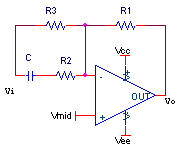
\includegraphics{schematics/activelead.PNG}
\end{center}
This is a fairly simple lead compensator which uses an operational amplifier to provide $K > 1$. It is the same as an inverting amplifier except that a capacitor and resistor in series are placed in parallel with the input resistor. The same analysis can be used as the one for the inverting amplifer except that the impedance from \vin to the op amp's inverting input is $R_3 \parallel (R_2 + \frac{1}{Cs})$. The transfer function \autocite[278]{analog-design-feedback-lundberg} is thus

\textcolor{red}{
\begin{equation}
\frac{\vout}{\vin}(s) = -\frac{R_1}{R_3}\frac{1+s(R_2 + R_3)C}{1+sR_2C}
\label{eq:activelead}
\end{equation}
}

\section{Type I active compensator}
\begin{center}
	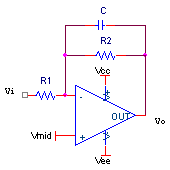
\includegraphics{schematics/type1compensator.PNG}
\end{center}
This compensator is essentially a low pass filter since it has a single pole and no zeroes. It can be used to lower the plant's gain at higher frequencies exactly as a low pass filter and thus improve high frequency noise rejection, or it can be used a dominant pole compensator if the DC gain $\frac{R_{2}}{R_{1}}$ is chosen sufficiently high and the compensator's pole is chosen to be a sufficiently low frequency. The transfer function is the same as that of an op amp in an inverting amplifier configuration, except that the feedback impedance is
\begin{equation}
R_{2}||C = \frac{R_{2}}{1+sR_{2}C}
\end{equation}

Thus it is

\textcolor{red}{
\begin{equation}
\frac{v_{o}}{v_{i}}(s) = -\frac{R_{2}}{R_{1}}\frac{1}{1+sR_{2}C}
\label{eq:type1compensator}
\end{equation}
}

\section{Type II active compensator}
\begin{center}
	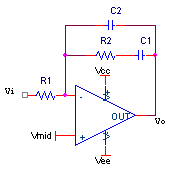
\includegraphics{schematics/type2compensator.PNG}
\end{center}
This compensator is a bit more complex: it has a zero, a pole at the origin, and a second pole. The pole at the origin is caused by the two capacitors in the feedback path; since both are open circuits at DC there is no feedback path at DC and the DC gain is the op amp's open loop gain. To derive the transfer function use the fact that the op amp is configured as an inverting amplifier but with a feedback impedance of
\begin{equation}
\left(R_{2}+\frac{1}{sC_{1}}\right)||\frac{1}{sC_{2}} = \frac{1+sR_{2}C_{1}}{s(sR_{2}C_{1}C_{2}+C_{1}+C_{2})}
\end{equation}

Dividing this impedance by $-\frac{1}{R_{1}}$ and rearranging, we see the transfer function is

\textcolor{red}{
\begin{equation}
\frac{v_{o}}{v_{i}}(s) = -\frac{1+sR_{2}C_{1}}{sR_{1}(C_{1}+C_{2})(1+sR_{2}\frac{C_{1}C_{2}}{C_{1}+C_{2}})}
\label{eq:type2compensator}
\end{equation}
}

\section{Type III active compensator}
\begin{center}
	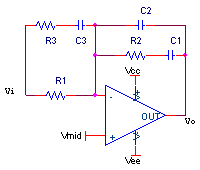
\includegraphics{schematics/type3compensator.PNG}
\end{center}
This compensator is even more complex because it adds a resistor and capacitor to the input network and in doing so adds another zero and pole for a total of two zeroes, a pole at the origin, and two additional poles. So many zeroes and poles make this a very flexible compensator that can significantly improve a plant's transfer function, but at the cost of complexity. Fortunately, we have already done most of the work in deriving the transfer function since this compensator's feedback network is the same as that of the type II compensator above. The input network is now
\begin{equation}
R_{1}||\left(R_{3}+\frac{1}{sC_{3}}\right) = \frac{R_{1}(1+sR_{3}C_{3})}{1+s(R_{1}+R_{3})C_{3}}
\end{equation}

and so the transfer function is

\textcolor{red}{
\begin{equation}
\frac{v_{o}}{v_{i}}(s) = -\frac{(1+sR_{2}C_{1})(1+s(R_{1}+R_{3})C_{3})}{sR_{1}(C_{1}+C_{2})(1+sR_{3}C_{3})(1+sR_{2}\frac{C_{1}C_{2}}{C_{1}+C_{2}})}
\label{eq:type3compensator}
\end{equation}
}